\documentclass{standalone}
\usepackage{tikz}
\usetikzlibrary{patterns}
\usetikzlibrary{positioning}
\usetikzlibrary{patterns, positioning}
\usetikzlibrary{shapes.misc}
\usepackage[outline]{contour}
\contourlength{1.5pt} 
\usepackage[sfdefault]{ClearSans}

\begin{document}
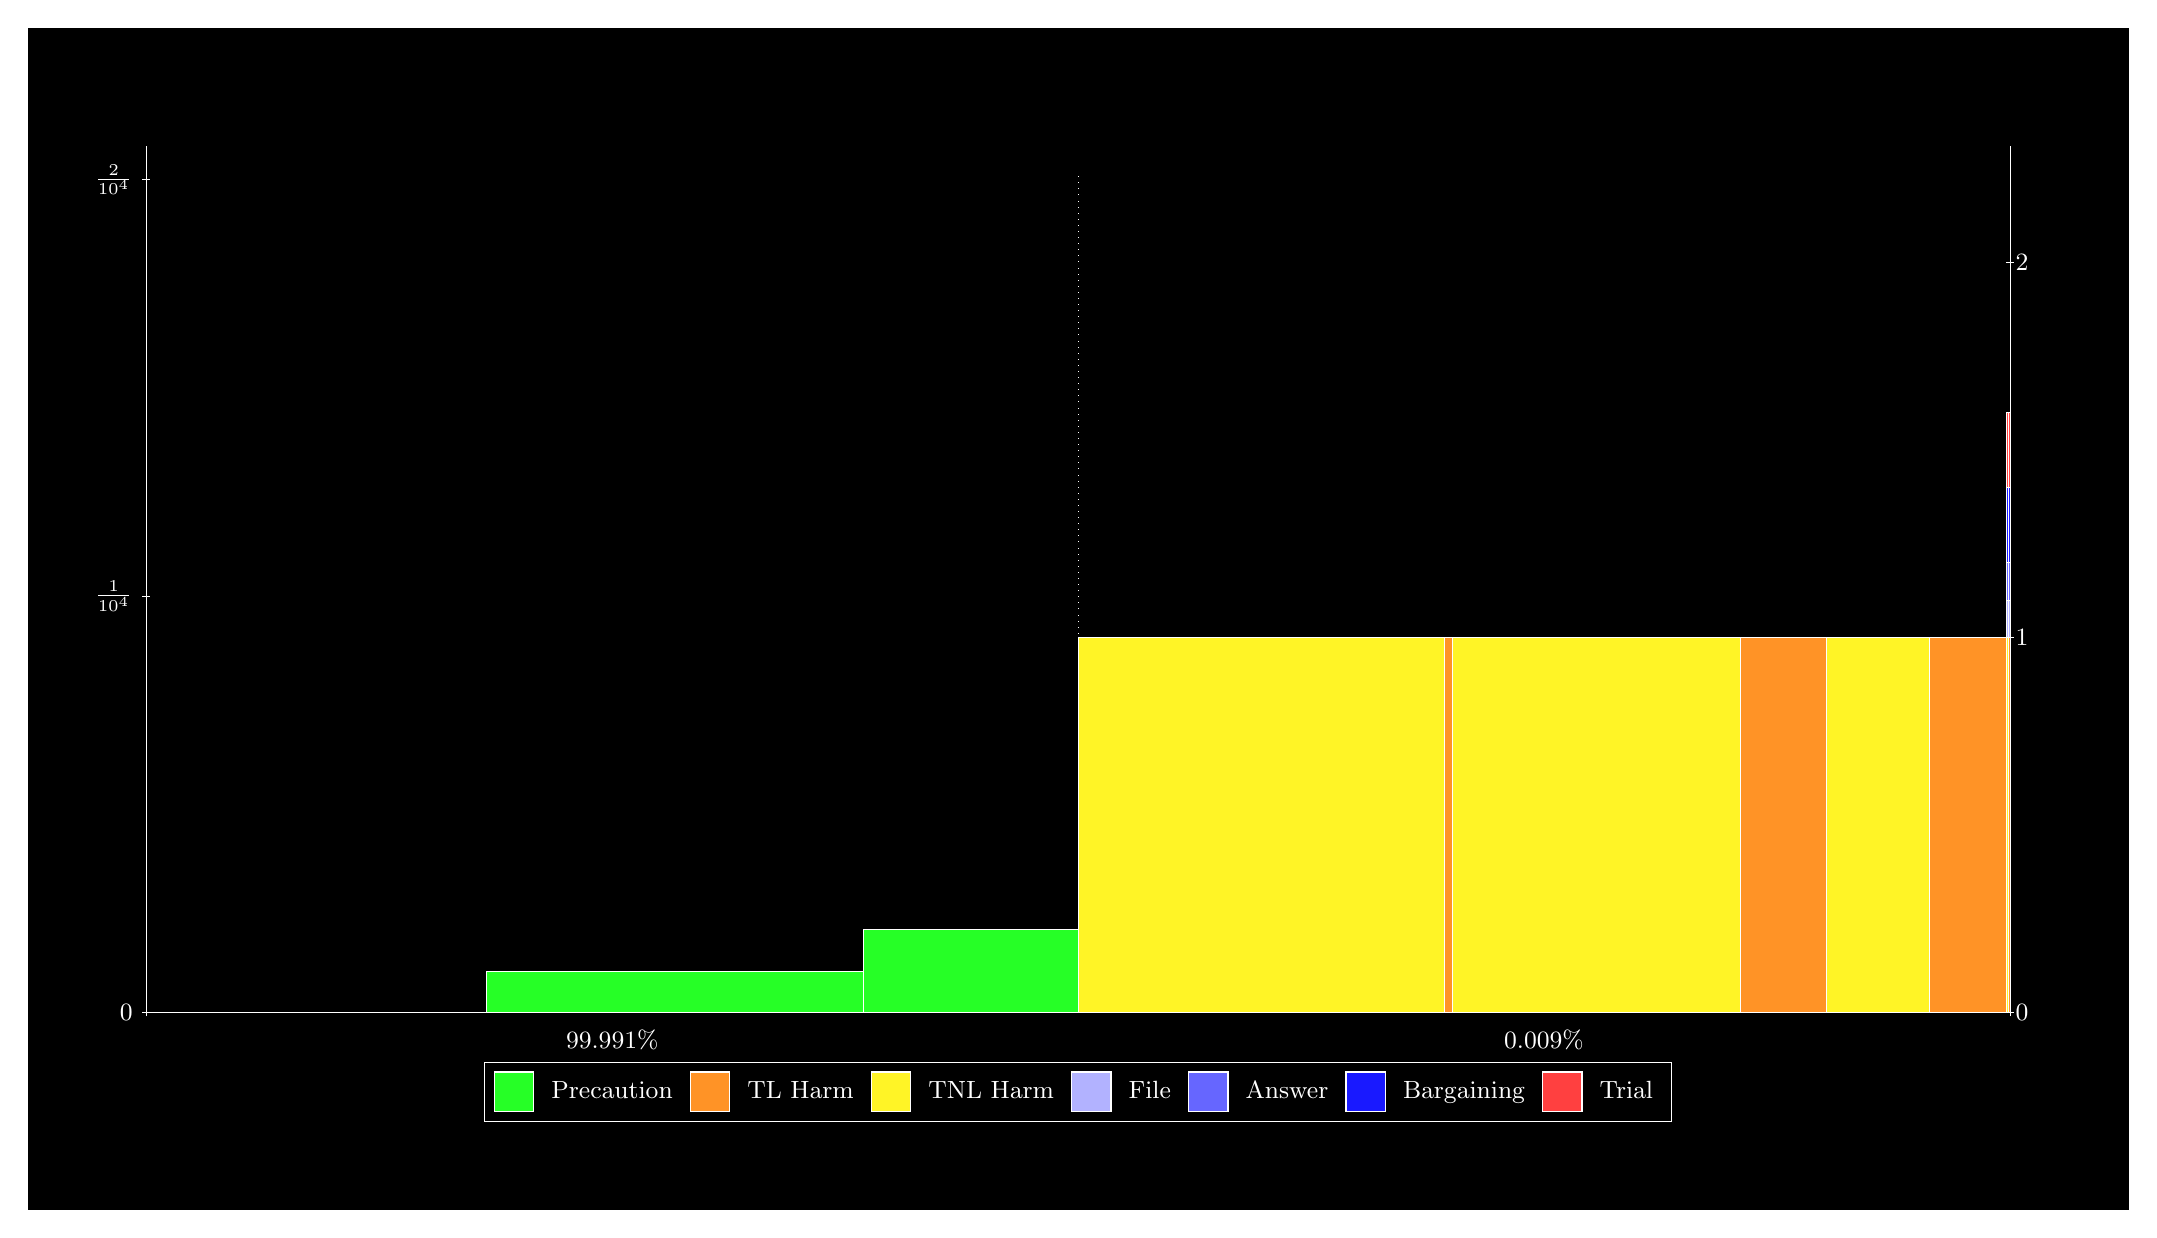
\begin{tikzpicture}
\draw[fill=black] (0,0) rectangle (26.667,15);
\draw[fill=green!85,draw=white,very thin] (5.8206,2.5) rectangle (10.611,3.0289);
\draw[fill=green!85,draw=white,very thin] (10.611,2.5) rectangle (13.333,3.5578);
\draw[fill=blue!30,draw=white,very thin] (13.333,2.5) rectangle (13.338,2.9762);
\draw[fill=blue!60,draw=white,very thin] (13.333,2.9762) rectangle (13.338,3.4525);
\draw[fill=blue!90,draw=white,very thin] (13.333,3.4525) rectangle (13.338,4.405);
\draw[fill=red!75,draw=white,very thin] (13.333,4.405) rectangle (13.338,5.3575);
\draw[fill=yellow!85,draw=white,very thin] (13.338,2.5) rectangle (17.983,7.2625);
\draw[fill=orange!85,draw=white,very thin] (17.983,2.5) rectangle (18.091,7.2625);
\draw[fill=green!85,draw=white,very thin] (18.091,2.5) rectangle (21.741,2.5);
\draw[fill=yellow!85,draw=white,very thin] (18.091,2.5) rectangle (21.741,7.2625);
\draw[fill=green!85,draw=white,very thin] (21.741,2.5) rectangle (22.837,2.5);
\draw[fill=orange!85,draw=white,very thin] (21.741,2.5) rectangle (22.837,7.2625);
\draw[fill=green!85,draw=white,very thin] (22.837,2.5) rectangle (24.148,2.5001);
\draw[fill=yellow!85,draw=white,very thin] (22.837,2.5001) rectangle (24.148,7.2626);
\draw[fill=green!85,draw=white,very thin] (24.148,2.5) rectangle (25.121,2.5001);
\draw[fill=orange!85,draw=white,very thin] (24.148,2.5001) rectangle (25.121,7.2626);
\draw[fill=yellow!85,draw=white,very thin] (25.121,2.5) rectangle (25.144,7.2625);
\draw[fill=blue!30,draw=white,very thin] (25.121,7.2625) rectangle (25.144,7.7387);
\draw[fill=blue!60,draw=white,very thin] (25.121,7.7387) rectangle (25.144,8.215);
\draw[fill=blue!90,draw=white,very thin] (25.121,8.215) rectangle (25.144,9.1675);
\draw[fill=red!75,draw=white,very thin] (25.121,9.1675) rectangle (25.144,10.12);
\draw[fill=orange!85,draw=white,very thin] (25.144,2.5) rectangle (25.167,7.2625);
\draw[fill=blue!30,draw=white,very thin] (25.144,7.2625) rectangle (25.167,7.7387);
\draw[fill=blue!60,draw=white,very thin] (25.144,7.7387) rectangle (25.167,8.215);
\draw[fill=blue!90,draw=white,very thin] (25.144,8.215) rectangle (25.167,9.1675);
\draw[fill=red!75,draw=white,very thin] (25.144,9.1675) rectangle (25.167,10.12);
\draw[white,very thin] (1.5,2.5) -- (1.5,13.5);
\draw[white,very thin] (1.45,2.5) -- (1.55,2.5);
\node[font=\small,text=white, anchor=east] at (1.45, 2.5) {0};
\draw[white,very thin] (1.45,7.7892) -- (1.55,7.7892);
\node[font=\small,text=white, anchor=east] at (1.45, 7.7892) {$\frac{1}{10^{4}}$};
\draw[white,very thin] (1.45,13.078) -- (1.55,13.078);
\node[font=\small,text=white, anchor=east] at (1.45, 13.078) {$\frac{2}{10^{4}}$};

\draw[white,dotted,very thin] (13.333,2.83) -- (13.333,13.17);
\draw[white,very thin] (25.167,2.5) -- (25.167,13.5);
\draw[white,very thin] (25.117,2.5) -- (25.217,2.5);
\node[font=\small,text=white, anchor=west] at (25.117, 2.5) {0};
\draw[white,very thin] (25.117,7.2625) -- (25.217,7.2625);
\node[font=\small,text=white, anchor=west] at (25.117, 7.2625) {1};
\draw[white,very thin] (25.117,12.025) -- (25.217,12.025);
\node[font=\small,text=white, anchor=west] at (25.117, 12.025) {2};

\draw[white,very thin] (1.5,2.5) -- (25.167,2.5);
\draw[white,very thin] (1.5,2.45) -- (1.5,2.55);
\node[font=\small,text=white, anchor=north] at (1.5, 2.45) {};
\draw[white,very thin] (25.167,2.45) -- (25.167,2.55);
\node[font=\small,text=white, anchor=north] at (25.167, 2.45) {};

\node[font=\small,text=white,anchor=south] at (7.4167, 1.9) {99.991\%};
\node[font=\small,text=white,anchor=south] at (19.25, 1.9) {0.009\%};
\draw (13.3333,2.5) node (B) {};
\begin{scope}[align=center]
\matrix[scale=0.5,draw=white,below=0.5cm of B,nodes={draw},column sep=0.1cm]{
\node[rectangle,draw,minimum width=0.5cm,minimum height=0.5cm,fill=green!85]{}; & \node[draw=none,font=\small,text=white]{Precaution}; &
\node[rectangle,draw,minimum width=0.5cm,minimum height=0.5cm,fill=orange!85]{}; & \node[draw=none,font=\small,text=white]{TL Harm}; &
\node[rectangle,draw,minimum width=0.5cm,minimum height=0.5cm,fill=yellow!85]{}; & \node[draw=none,font=\small,text=white]{TNL Harm}; &
\node[rectangle,draw,minimum width=0.5cm,minimum height=0.5cm,fill=blue!30]{}; & \node[draw=none,font=\small,text=white]{File}; &
\node[rectangle,draw,minimum width=0.5cm,minimum height=0.5cm,fill=blue!60]{}; & \node[draw=none,font=\small,text=white]{Answer}; &
\node[rectangle,draw,minimum width=0.5cm,minimum height=0.5cm,fill=blue!90]{}; & \node[draw=none,font=\small,text=white]{Bargaining}; &
\node[rectangle,draw,minimum width=0.5cm,minimum height=0.5cm,fill=red!75]{}; & \node[draw=none,font=\small,text=white]{Trial}; \\\\
};\end{scope}

\end{tikzpicture}
\end{document}